
\documentclass[letterpaper,hide notes,xcolor={table,svgnames},pdftex,10pt]{beamer}
\def\showexamples{t}


%\usepackage[svgnames]{xcolor}

%% Demo talk
%\documentclass[letterpaper,notes=show]{beamer}

\usecolortheme{crane}
\setbeamertemplate{navigation symbols}{}

\usetheme{MyPittsburgh}
%\usetheme{Frankfurt}

%\usepackage{tipa}

\usepackage{hyperref}
\usepackage{graphicx,xspace}
\usepackage[normalem]{ulem}
\usepackage{multicol}
\usepackage{amsmath,amssymb,amsthm,graphicx,xspace}
\newcommand\SF[1]{$\bigstar$\footnote{SF: #1}}

\usepackage[default]{sourcesanspro}
\usepackage[T1]{fontenc}
\usepackage[scaled]{beramono}
\usepackage{tikzpagenodes}

\newcounter{tmpnumSlide}
\newcounter{tmpnumNote}


% old question code
%\newcommand\question[1]{{$\bigstar$ \small \onlySlide{2}{#1}}}
% \newcommand\nquestion[1]{\ifdefined \presentationonly \textcircled{?} \fi \note{\par{\Large \textbf{?}} #1}}
% \newcommand\nanswer[1]{\note{\par{\Large \textbf{A}} #1}}


 \newcommand\mnote[1]{%
   \addtocounter{tmpnumSlide}{1}
   \ifdefined\showcues {~\tiny\fbox{\arabic{tmpnumSlide}}}\fi
   \note{\setlength{\parskip}{1ex}\addtocounter{tmpnumNote}{1}\textbf{\Large \arabic{tmpnumNote}:} {#1\par}}}

\newcommand\mmnote[1]{\note{\setlength{\parskip}{1ex}#1\par}}

%\newcommand\mnote[2][]{\ifdefined\handoutwithnotes {~\tiny\fbox{#1}}\fi
% \note{\setlength{\parskip}{1ex}\textbf{\Large #1:} #2\par}}

%\newcommand\mnote[2][]{{\tiny\fbox{#1}} \note{\setlength{\parskip}{1ex}\textbf{\Large #1:} #2\par}}

\newcommand\mquestion[2]{{~\color{red}\fbox{?}}\note{\setlength{\parskip}{1ex}\par{\Large \textbf{?}} #1} \note{\setlength{\parskip}{1ex}\par{\Large \textbf{A}} #2\par}\ifdefined \presentationonly \pause \fi}

\newcommand\blackboard[1]{%
\ifdefined   \showblackboard
  {#1}
  \else {\begin{center} \fbox{\colorbox{blue!30}{%
         \begin{minipage}{.95\linewidth}%
           \hspace{\stretch{1}} Some space intentionally left blank; done at the blackboard.%
         \end{minipage}}}\end{center}}%
         \fi%
}



%\newcommand\q{\tikz \node[thick,color=black,shape=circle]{?};}
%\newcommand\q{\ifdefined \presentationonly \textcircled{?} \fi}

\usepackage{listings}
\lstset{basicstyle=\footnotesize\ttfamily,
	breaklines=true,
	aboveskip=15pt,
  	belowskip=15pt,
	frame=lines,
	numbers=left, basicstyle=\scriptsize, numberstyle=\tiny, stepnumber=0, numbersep=2pt
}

\usepackage{siunitx}
\newcommand\sius[1]{\num[group-separator = {,}]{#1}\si{\micro\second}}
\newcommand\sims[1]{\num[group-separator = {,}]{#1}\si{\milli\second}}
\newcommand\sins[1]{\num[group-separator = {,}]{#1}\si{\nano\second}}
\sisetup{group-separator = {,}, group-digits = true}

%% -------------------- tikz --------------------
\usepackage{tikz}
\usetikzlibrary{positioning}
\usetikzlibrary{arrows,backgrounds,automata,decorations.shapes,decorations.pathmorphing,decorations.markings,decorations.text,decorations.pathreplacing}

\tikzstyle{place}=[circle,draw=blue!50,fill=blue!20,thick, inner sep=0pt,minimum size=6mm]
\tikzstyle{transition}=[rectangle,draw=black!50,fill=black!20,thick, inner sep=0pt,minimum size=4mm]

\tikzstyle{block}=[rectangle,draw=black, thick, inner sep=5pt]
\tikzstyle{bullet}=[circle,draw=black, fill=black, thin, inner sep=2pt]

\tikzstyle{pre}=[<-,shorten <=1pt,>=stealth',semithick]
\tikzstyle{post}=[->,shorten >=1pt,>=stealth',semithick]
\tikzstyle{bi}=[<->,shorten >=1pt,shorten <=1pt, >=stealth',semithick]

\tikzstyle{mut}=[-,>=stealth',semithick]

\tikzstyle{treereset}=[dashed,->, shorten >=1pt,>=stealth',thin]

\usepackage{ifmtarg}
\usepackage{xifthen}
\makeatletter
% new counter to now which frame it is within the sequence
\newcounter{multiframecounter}
% initialize buffer for previously used frame title
\gdef\lastframetitle{\textit{undefined}}
% new environment for a multi-frame
\newenvironment{multiframe}[1][]{%
\ifthenelse{\isempty{#1}}{%
% if no frame title was set via optional parameter,
% only increase sequence counter by 1
\addtocounter{multiframecounter}{1}%
}{%
% new frame title has been provided, thus
% reset sequence counter to 1 and buffer frame title for later use
\setcounter{multiframecounter}{1}%
\gdef\lastframetitle{#1}%
}%
% start conventional frame environment and
% automatically set frame title followed by sequence counter
\begin{frame}%
\frametitle{\lastframetitle~{\normalfont(\arabic{multiframecounter})}}%
}{%
\end{frame}%
}
\makeatother

\makeatletter
\newdimen\tu@tmpa%
\newdimen\ydiffl%
\newdimen\xdiffl%
\newcommand\ydiff[2]{%
    \coordinate (tmpnamea) at (#1);%
    \coordinate (tmpnameb) at (#2);%
    \pgfextracty{\tu@tmpa}{\pgfpointanchor{tmpnamea}{center}}%
    \pgfextracty{\ydiffl}{\pgfpointanchor{tmpnameb}{center}}%
    \advance\ydiffl by -\tu@tmpa%
}
\newcommand\xdiff[2]{%
    \coordinate (tmpnamea) at (#1);%
    \coordinate (tmpnameb) at (#2);%
    \pgfextractx{\tu@tmpa}{\pgfpointanchor{tmpnamea}{center}}%
    \pgfextractx{\xdiffl}{\pgfpointanchor{tmpnameb}{center}}%
    \advance\xdiffl by -\tu@tmpa%
}
\makeatother
\newcommand{\copyrightbox}[3][r]{%
\begin{tikzpicture}%
\node[inner sep=0pt,minimum size=2em](ciimage){#2};
\usefont{OT1}{phv}{n}{n}\fontsize{4}{4}\selectfont
\ydiff{ciimage.south}{ciimage.north}
\xdiff{ciimage.west}{ciimage.east}
\ifthenelse{\equal{#1}{r}}{%
\node[inner sep=0pt,right=1ex of ciimage.south east,anchor=north west,rotate=90]%
{\raggedleft\color{black!50}\parbox{\the\ydiffl}{\raggedright{}#3}};%
}{%
\ifthenelse{\equal{#1}{l}}{%
\node[inner sep=0pt,right=1ex of ciimage.south west,anchor=south west,rotate=90]%
{\raggedleft\color{black!50}\parbox{\the\ydiffl}{\raggedright{}#3}};%
}{%
\node[inner sep=0pt,below=1ex of ciimage.south west,anchor=north west]%
{\raggedleft\color{black!50}\parbox{\the\xdiffl}{\raggedright{}#3}};%
}
}
\end{tikzpicture}
}


%% --------------------

%\usepackage[excludeor]{everyhook}
%\PushPreHook{par}{\setbox0=\lastbox\llap{MUH}}\box0}

%\vspace*{\stretch{1}

%\setbox0=\lastbox \llap{\textbullet\enskip}\box0}

\setlength{\parskip}{\fill}

\newcommand\noskips{\setlength{\parskip}{1ex}}
\newcommand\doskips{\setlength{\parskip}{\fill}}

\newcommand\xx{\par\vspace*{\stretch{1}}\par}
\newcommand\xxs{\par\vspace*{2ex}\par}
\newcommand\tuple[1]{\langle #1 \rangle}
\newcommand\code[1]{{\sf \footnotesize #1}}
\newcommand\ex[1]{\uline{Example:} \ifdefined \presentationonly \pause \fi
  \ifdefined\showexamples#1\xspace\else{\uline{\hspace*{2cm}}}\fi}

\newcommand\ceil[1]{\lceil #1 \rceil}


\AtBeginSection[]
{
   \begin{frame}
       \frametitle{Outline}
       \tableofcontents[currentsection]
   \end{frame}
}



\pgfdeclarelayer{edgelayer}
\pgfdeclarelayer{nodelayer}
\pgfsetlayers{edgelayer,nodelayer,main}

\tikzstyle{none}=[inner sep=0pt]
\tikzstyle{rn}=[circle,fill=Red,draw=Black,line width=0.8 pt]
\tikzstyle{gn}=[circle,fill=Lime,draw=Black,line width=0.8 pt]
\tikzstyle{yn}=[circle,fill=Yellow,draw=Black,line width=0.8 pt]
\tikzstyle{empty}=[circle,fill=White,draw=Black]
\tikzstyle{bw} = [rectangle, draw, fill=blue!20, 
    text width=4em, text centered, rounded corners, minimum height=2em]
    
    \newcommand{\CcNote}[1]{% longname
	This work is licensed under the \textit{Creative Commons #1 3.0 License}.%
}
\newcommand{\CcImageBy}[1]{%
	\includegraphics[scale=#1]{creative_commons/cc_by_30.pdf}%
}
\newcommand{\CcImageSa}[1]{%
	\includegraphics[scale=#1]{creative_commons/cc_sa_30.pdf}%
}
\newcommand{\CcImageNc}[1]{%
	\includegraphics[scale=#1]{creative_commons/cc_nc_30.pdf}%
}
\newcommand{\CcGroupBySa}[2]{% zoom, gap
	\CcImageBy{#1}\hspace*{#2}\CcImageNc{#1}\hspace*{#2}\CcImageSa{#1}%
}
\newcommand{\CcLongnameByNcSa}{Attribution-NonCommercial-ShareAlike}

\newenvironment{changemargin}[1]{% 
  \begin{list}{}{% 
    \setlength{\topsep}{0pt}% 
    \setlength{\leftmargin}{#1}% 
    \setlength{\rightmargin}{1em}
    \setlength{\listparindent}{\parindent}% 
    \setlength{\itemindent}{\parindent}% 
    \setlength{\parsep}{\parskip}% 
  }% 
  \item[]}{\end{list}} 




\title{Lecture 25 --- System-Level Profiling, Profiler Guided Optimization }

\author{Patrick Lam \& Jeff Zarnett \\ \small \texttt{patrick.lam@uwaterloo.ca}, \texttt{jzarnett@uwaterloo.ca}}
\institute{Department of Electrical and Computer Engineering \\
  University of Waterloo}
\date{\today}


\begin{document}

\begin{frame}
  \titlepage

 \end{frame}

%%%%%%%%%%%%%%%%%%%%%%%%%%%%%%%%%%%%%%%%%%%%%%%%%%%%%%%%%%%%%%%%%%%%%%%%%%%%%%%%


% How to Read
% http://www.cs.utah.edu/dept/old/texinfo/as/gprof.html
% http://www.civilnet.cn/book/kernel/GNU.Linux.Application.Programming/LiB0055.html
% http://ececmpsysweb.groups.et.byu.net/cmpsys.2004.winter/citizenship/Bryan_Wheeler/Profiling_Tutorial.html

% gprof
% OProfile
% Valgrind
% Intel VTune
% AMD CodeAnalyst


%%%%%%%%%%%%%%%%%%%%%%%%%%%%%%%%%%%%%%%%%%%%%%%%%%%%%%%%%%%%%%%%%%%%%%%%%%%%%%%%
\begin{frame}
  \frametitle{Introduction: oprofile}

\large
\begin{changemargin}{1.5cm}

    \url{http://oprofile.sourceforge.net}\\[1em]

    Sampling-based tool.\\[1em]
    
    Uses CPU performance counters.\\[1em]

    Tracks currently-running function;\\
    records profiling data for every application run.\\[1em]

    Can work system-wide (across processes).\\[1em]

    Technology: Linux Kernel Performance Events\\ (formerly a Linux kernel module).
    \end{changemargin}
\end{frame}
%%%%%%%%%%%%%%%%%%%%%%%%%%%%%%%%%%%%%%%%%%%%%%%%%%%%%%%%%%%%%%%%%%%%%%%%%%%%%%%%

%%%%%%%%%%%%%%%%%%%%%%%%%%%%%%%%%%%%%%%%%%%%%%%%%%%%%%%%%%%%%%%%%%%%%%%%%%%%%%%%
\begin{frame}[fragile]
  \frametitle{Setting up {\tt oprofile}}

\large
\begin{changemargin}{1.5cm}

  Must run as root to use system-wide, \\
otherwise can use per-process.

  \begin{lstlisting}
% sudo opcontrol \
     --vmlinux=/usr/src/linux-3.2.7-1-ARCH/vmlinux
% echo 0 | sudo tee /proc/sys/kernel/nmi_watchdog
% sudo opcontrol --start
Using default event: CPU_CLK_UNHALTED:100000:0:1:1
Using 2.6+ OProfile kernel interface.
Reading module info.
Using log file /var/lib/oprofile/samples/oprofiled.log
Daemon started.
Profiler running.
  \end{lstlisting}

  Per-process:
\begin{lstlisting}
[plam@lynch nm-morph]$ operf ./test_harness
operf: Profiler started

Profiling done.
\end{lstlisting}%$
\end{changemargin}

\end{frame}
%%%%%%%%%%%%%%%%%%%%%%%%%%%%%%%%%%%%%%%%%%%%%%%%%%%%%%%%%%%%%%%%%%%%%%%%%%%%%%%%

%%%%%%%%%%%%%%%%%%%%%%%%%%%%%%%%%%%%%%%%%%%%%%%%%%%%%%%%%%%%%%%%%%%%%%%%%%%%%%%%
\begin{frame}[fragile]
  \frametitle{{\tt oprofile} Usage (1)}
  

\large
\begin{changemargin}{1.5cm}
  Pass your executable to {\tt opreport}.

  \begin{lstlisting}
% sudo opreport -l ./test    
CPU: Intel Core/i7, speed 1595.78 MHz (estimated)
Counted CPU_CLK_UNHALTED events (Clock cycles when not
halted) with a unit mask of 0x00 (No unit mask) count 100000
samples  %        symbol name
7550     26.0749  int_math_helper
5982     20.6596  int_power
5859     20.2348  float_power
3605     12.4504  float_math
3198     11.0447  int_math
2601      8.9829  float_math_helper
160       0.5526  main
  \end{lstlisting}
  
    If you have debug symbols ({\tt -g}) you could use:

  \begin{lstlisting}
% sudo opannotate --source \
--output-dir=/path/to/annotated-source /path/to/mybinary
  \end{lstlisting}
  \end{changemargin}
\end{frame}
%%%%%%%%%%%%%%%%%%%%%%%%%%%%%%%%%%%%%%%%%%%%%%%%%%%%%%%%%%%%%%%%%%%%%%%%%%%%%%%%

%%%%%%%%%%%%%%%%%%%%%%%%%%%%%%%%%%%%%%%%%%%%%%%%%%%%%%%%%%%%%%%%%%%%%%%%%%%%%%%%
\begin{frame}[fragile]
  \frametitle{{\tt oprofile} Usage (2)}
  

\large
\begin{changemargin}{1.5cm}
    Use {\tt opreport} by itself for a whole-system view.\\
    You can also reset and stop the profiling.

  \begin{lstlisting}
% sudo opcontrol --reset 
Signalling daemon... done
% sudo opcontrol --stop
Stopping profiling.
  \end{lstlisting}
  \end{changemargin}
\end{frame}
%%%%%%%%%%%%%%%%%%%%%%%%%%%%%%%%%%%%%%%%%%%%%%%%%%%%%%%%%%%%%%%%%%%%%%%%%%%%%%%%

%%%%%%%%%%%%%%%%%%%%%%%%%%%%%%%%%%%%%%%%%%%%%%%%%%%%%%%%%%%%%%%%%%%%%%%%%%%%%%%%
\begin{frame}
  \frametitle{Perf: Introduction}

\large
\begin{changemargin}{1cm}

    \url{perf.wiki.kernel.org/index.php/Tutorial}\\[1em]

    Interface to Linux kernel built-in sampling-based profiling.\\
    Per-process, per-CPU, or system-wide.\\
    Can even report the cost of each line of code.
    \end{changemargin}
\end{frame}
%%%%%%%%%%%%%%%%%%%%%%%%%%%%%%%%%%%%%%%%%%%%%%%%%%%%%%%%%%%%%%%%%%%%%%%%%%%%%%%%

%%%%%%%%%%%%%%%%%%%%%%%%%%%%%%%%%%%%%%%%%%%%%%%%%%%%%%%%%%%%%%%%%%%%%%%%%%%%%%%%
\begin{frame}[fragile]
  \frametitle{Perf: Usage Example}

\large
\begin{changemargin}{1.5cm}
On previous Assignment 3 code:
\begin{lstlisting}[basicstyle=\tiny]
[plam@lynch nm-morph]$ perf stat ./test_harness

 Performance counter stats for './test_harness':

       6562.501429 task-clock                #    0.997 CPUs utilized          
               666 context-switches          #    0.101 K/sec                  
                 0 cpu-migrations            #    0.000 K/sec                  
             3,791 page-faults               #    0.578 K/sec                  
    24,874,267,078 cycles                    #    3.790 GHz                     [83.32%]
    12,565,457,337 stalled-cycles-frontend   #   50.52% frontend cycles idle    [83.31%]
     5,874,853,028 stalled-cycles-backend    #   23.62% backend  cycles idle    [66.63%]
    33,787,408,650 instructions              #    1.36  insns per cycle        
                                             #    0.37  stalled cycles per insn [83.32%]
     5,271,501,213 branches                  #  803.276 M/sec                   [83.38%]
       155,568,356 branch-misses             #    2.95% of all branches         [83.36%]

       6.580225847 seconds time elapsed
\end{lstlisting} %$
\end{changemargin}
\end{frame}
%%%%%%%%%%%%%%%%%%%%%%%%%%%%%%%%%%%%%%%%%%%%%%%%%%%%%%%%%%%%%%%%%%%%%%%%%%%%%%%%

%%%%%%%%%%%%%%%%%%%%%%%%%%%%%%%%%%%%%%%%%%%%%%%%%%%%%%%%%%%%%%%%%%%%%%%%%%%%%%%%
\begin{frame}[fragile]
  \frametitle{Perf: Source-level Analysis}


\large
\begin{changemargin}{1.5cm}
perf can tell you which instructions are taking time, or which lines of code.\\[1em]

Compile with {\tt -ggdb} to enable source code viewing.

\begin{lstlisting}
% perf record ./test_harness
% perf annotate
\end{lstlisting}

{\tt perf annotate} is interactive. Play around with it.
\end{changemargin}

\end{frame}
%%%%%%%%%%%%%%%%%%%%%%%%%%%%%%%%%%%%%%%%%%%%%%%%%%%%%%%%%%%%%%%%%%%%%%%%%%%%%%%%

%%%%%%%%%%%%%%%%%%%%%%%%%%%%%%%%%%%%%%%%%%%%%%%%%%%%%%%%%%%%%%%%%%%%%%%%%%%%%%%%
\begin{frame}
  \frametitle{DTrace: Introduction}

\large
\begin{changemargin}{1.5cm}
\vspace*{-4em}
    \url{http://queue.acm.org/detail.cfm?id=1117401}\\
    \url{http://www.brendangregg.com/blog/2016-10-27/dtrace-for-linux-2016.html}\\[1em]

    Intrumentation-based tool.\\
    System-wide.\\
    Meant to be used on production systems. (Eh?)\\[1em]
     \only<2>{
     {\small (Typical instrumentation can have a slowdown of 100x (Valgrind).)}\\
     Design goals:\\
\begin{enumerate} 
\item No overhead when not in use;
\item Guarantee safety---must not crash\\ \qquad (strict limits on expressiveness of probes).
\end{enumerate}
     }
     \end{changemargin}
\end{frame}
%%%%%%%%%%%%%%%%%%%%%%%%%%%%%%%%%%%%%%%%%%%%%%%%%%%%%%%%%%%%%%%%%%%%%%%%%%%%%%%%

%%%%%%%%%%%%%%%%%%%%%%%%%%%%%%%%%%%%%%%%%%%%%%%%%%%%%%%%%%%%%%%%%%%%%%%%%%%%%%%%
\begin{frame}
  \frametitle{DTrace: Operation}

\large
\begin{changemargin}{1.5cm}

    How does DTrace achieve 0 overhead?\\
\begin{itemize}
    \item only when activated, dynamically rewrites code by placing a branch to
      instrumentation code.
\end{itemize}

    Uninstrumented: runs as if nothing changed.\\[1em]

    Most instrumentation: at function entry or exit points.\\
    You can also instrument kernel functions, locking, instrument-based
      on other events.\\[1em]

    Can express sampling as instrumentation-based events also.
    \end{changemargin}
\end{frame}
%%%%%%%%%%%%%%%%%%%%%%%%%%%%%%%%%%%%%%%%%%%%%%%%%%%%%%%%%%%%%%%%%%%%%%%%%%%%%%%%

%%%%%%%%%%%%%%%%%%%%%%%%%%%%%%%%%%%%%%%%%%%%%%%%%%%%%%%%%%%%%%%%%%%%%%%%%%%%%%%%
\begin{frame}[fragile]
  \frametitle{DTrace Example}

\large
\begin{changemargin}{1cm}

  You write this:

  \begin{lstlisting}
syscall::read:entry {
    self->t = timestamp;
}

syscall::read:return
/self->t/ {
    printf("%d/%d spent %d nsecs in read\n"
           pid, tid, timestamp - self->t);
}
  \end{lstlisting}

    {\tt t} is a thread-local variable.\\
    This code prints how long each call to {\tt read} takes, along with
      context.\\[1em]
    To ensure safety, DTrace limits expressiveness---no loops.
      \begin{itemize}
        \item (Hence, no infinite loops!)
      \end{itemize}
      \end{changemargin}

\end{frame}
%%%%%%%%%%%%%%%%%%%%%%%%%%%%%%%%%%%%%%%%%%%%%%%%%%%%%%%%%%%%%%%%%%%%%%%%%%%%%%%%

%%%%%%%%%%%%%%%%%%%%%%%%%%%%%%%%%%%%%%%%%%%%%%%%%%%%%%%%%%%%%%%%%%%%%%%%%%%%%%%%
\begin{frame}[fragile]
  \frametitle{Other Tools}

\large
\begin{changemargin}{1.5cm}

    AMD CodeAnalyst---based on oprofile; leverages AMD processor features.\\[1em]

    WAIT\\[0em]
      \begin{itemize}
        \item IBM's tool tells you what operations your JVM is waiting on while
          idle.
        \item Non-free and not available.
      \end{itemize}
      \end{changemargin}
\end{frame}
%%%%%%%%%%%%%%%%%%%%%%%%%%%%%%%%%%%%%%%%%%%%%%%%%%%%%%%%%%%%%%%%%%%%%%%%%%%%%%%%

%%%%%%%%%%%%%%%%%%%%%%%%%%%%%%%%%%%%%%%%%%%%%%%%%%%%%%%%%%%%%%%%%%%%%%%%%%%%%%%%
\begin{frame}
  \frametitle{WAIT: Introduction}

\large
\begin{changemargin}{1.5cm}

Built for production environments.\\[1em]

Specialized for profiling JVMs, \\uses JVM hooks to analyze idle time.\\[1em]

Sampling-based analysis; infrequent samples\\ (1--2 per minute!)
\end{changemargin}
\end{frame}

%%%%%%%%%%%%%%%%%%%%%%%%%%%%%%%%%%%%%%%%%%%%%%%%%%%%%%%%%%%%%%%%%%%%%%%%%%%%%%%%

%%%%%%%%%%%%%%%%%%%%%%%%%%%%%%%%%%%%%%%%%%%%%%%%%%%%%%%%%%%%%%%%%%%%%%%%%%%%%%%%
\begin{frame}
  \frametitle{WAIT: Operation}

\large
\begin{changemargin}{1.5cm}

  At each sample: records each thread's state,
\begin{itemize}
\item call stack;
\item participation in system locks.
\end{itemize}

  Enables WAIT to compute a ``wait state'' \\(using expert-written rules): \\
what the process is currently doing or waiting on, e.g.
\begin{itemize}
\item disk;
\item GC;
\item network; 
\item blocked; 
\item etc.
\end{itemize}
\end{changemargin}

\end{frame}

%%%%%%%%%%%%%%%%%%%%%%%%%%%%%%%%%%%%%%%%%%%%%%%%%%%%%%%%%%%%%%%%%%%%%%%%%%%%%%%%

%%%%%%%%%%%%%%%%%%%%%%%%%%%%%%%%%%%%%%%%%%%%%%%%%%%%%%%%%%%%%%%%%%%%%%%%%%%%%%%%
\begin{frame}
  \frametitle{WAIT: Workflow}

\large
\begin{changemargin}{1.5cm}

You:
\begin{itemize}
\item run your application;
\item collect data (using a script or manually); and 
\item upload the data to the server.
\end{itemize}
Server provides
a report.\\
\begin{itemize}
\item You fix the performance problems.\\[1em]
\end{itemize}

Report indicates processor utilization (idle, your application, GC, 
etc); runnable threads; waiting threads (and why they are waiting); 
thread states; and a stack viewer.\\[1em]

Paper presents 6 case studies where WAIT identified performance
problems: deadlocks, server underloads, memory leaks, database
bottlenecks, and excess filesystem activity.

\end{changemargin}
\end{frame}
%%%%%%%%%%%%%%%%%%%%%%%%%%%%%%%%%%%%%%%%%%%%%%%%%%%%%%%%%%%%%%%%%%%%%%%%%%%%%%%%


%%%%%%%%%%%%%%%%%%%%%%%%%%%%%%%%%%%%%%%%%%%%%%%%%%%%%%%%%%%%%%%%%%%%%%%%%%%%%%%%
\begin{frame}[fragile]
  \frametitle{Other Profiling Tools}

  
\large
\begin{changemargin}{1.5cm}
    Profiling: Not limited to C/C++, or even code.\\[1em]

    You can profile Python using {\tt cProfile}; standard profiling technology.\\[1em]

    Google's Page Speed Tool: profiling for web pages---how can you make your page faster?\\
\begin{itemize}
\item reducing number of DNS lookups;
\item leveraging browser caching;
\item combining images;
\item plus, traditional JavaScript profiling.
\end{itemize}
\end{changemargin}
\end{frame}
%%%%%%%%%%%%%%%%%%%%%%%%%%%%%%%%%%%%%%%%%%%%%%%%%%%%%%%%%%%%%%%%%%%%%%%%%%%%%%%%

\part{Profiler Guided Optimization}
\begin{frame}
\partpage
\end{frame}

\begin{frame}
\frametitle{Profiler Guided Optimization}

\Large
\begin{changemargin}{2cm}

Using static analysis, \\
the compiler makes its best predictions about runtime behaviour.

Example: branch prediction. 
\end{changemargin}

\end{frame}



\begin{frame}[fragile]
\frametitle{A Branch To Predict}
\begin{changemargin}{1.5cm}
\begin{lstlisting}[language=C,basicstyle=\large]
void whichBranchIsTaken(int a, int b)
{
    if (a < b) {
        puts("a is less than b.");
    } else {
        puts("b is >= a.");
    }
}
\end{lstlisting}
\end{changemargin}
\end{frame}

\begin{frame}[fragile]
\frametitle{A Virtual Call to Devirtualize}

\begin{changemargin}{2cm}
\begin{lstlisting}[language=C,basicstyle=\large]
void devirtualization(int count)
{
    for (int i = 0; i < count; i++)
    {
        (*p) (x, y);
    }
}
\end{lstlisting}
\end{changemargin}
\end{frame}

\begin{frame}[fragile]
\frametitle{A Switch to Predict}
\begin{changemargin}{2cm}
\begin{lstlisting}[language=C,basicstyle=\large]
void switchCaseExpansion(int i)
{
    switch (i)
    {
    case 1:
        puts("I took case 1.");
        break;
    case 2:
        puts("I took case 2.");
        break;
    }
}
\end{lstlisting}
\end{changemargin}
\end{frame}



\begin{frame}
\frametitle{Adapting to an Uncertain World}
\large
\begin{changemargin}{2cm}
How can we know where we go?
\begin{itemize}
\item could provide hints\ldots
\end{itemize}

Java HotSpot virtual machine: \\
updates predictions on the fly. 

So, just guess.\\
If wrong, the Just-in-Time compiler adjusts \& recompiles.

The compiler runs and it does its job and that's it; the program is never updated with newer predictions if more data becomes known.
\end{changemargin}

\end{frame}



\begin{frame}
\frametitle{Profiling Mitigates Uncertainty}

\large
\begin{changemargin}{2cm}
C: usually no adaptive runtime system.

POGO:
\begin{itemize}
\item observe actual runs;
\item predict the future.
\end{itemize}

So, we need multi-step compilation:
\begin{itemize}
\item compile with profiling;
\item run to collect data;
\item recompile with profiling data to optimize.
\end{itemize}

\end{changemargin}

\end{frame}



\begin{frame}
\frametitle{Step One: Measure}

\large
\begin{changemargin}{2cm}
First, generate an executable with instrumentation. 

The compiler inserts a bunch of probes into the generated code to record data. 
\begin{itemize}
\item Function entry probes;
\item Edge probes;
\item Value probes.
\end{itemize}

Result: instrumented executable \\
plus empty database file (for profiling data).
\end{changemargin}

\end{frame}



\begin{frame}
\frametitle{Step Two: Training Day}

\begin{center}
	
\includegraphics[width=0.6\textwidth]{images/training-day.jpg}
\end{center}

\end{frame}


\begin{frame}
\frametitle{Step Two: Training Day}
\large
\begin{changemargin}{2cm}

Second, run the instrumented executable.

Real-world scenarios are best.

Ideally, spend training time on perf-critical sections. 

Use as many runs as you can stand.
\end{changemargin}
\end{frame}



\begin{frame}
\frametitle{Step Two: Training Day}

\large
\begin{changemargin}{2cm}
Don't exercise every part of the program\\
(ain't SE 465 here!)

That would be counterproductive.

Usage data must match real world scenarios,\\
or compiler gets misfacts about what's important. 

Or you might end up teaching it that almost nothing
is important\ldots (``everything's on the exam!'')
\end{changemargin}

\end{frame}



\begin{frame}
\frametitle{Step Three: Recompile}

\large
\begin{changemargin}{2cm}
Finally, compile the program again.

Inputs: source plus training data.

Outputs: (you hope) a better output executable than\\
from static analysis alone.
\end{changemargin}

\end{frame}



\begin{frame}
\frametitle{Summary Graphic}

\begin{center}
	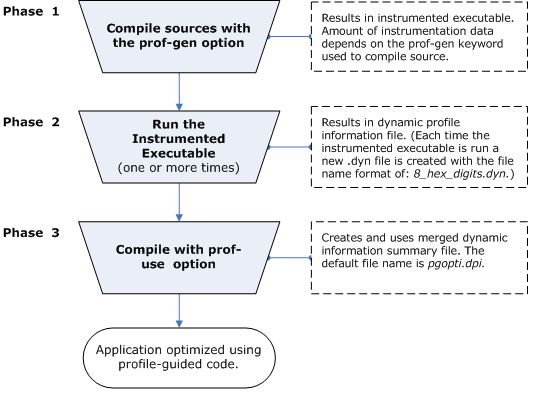
\includegraphics[width=0.75\textwidth]{images/pogo-workflow.jpg}
\end{center}

\end{frame}



\begin{frame}
\frametitle{Save Some Steps}

\large
\begin{changemargin}{2cm}
Not necessary to do all three steps for every build. 

Re-use training data while it's still valid.

Recommended dev workflow:
\begin{itemize}
\item dev A performs these steps, \\
checks the training data into source control
\item whole team can use profiling information for their compiles.
\end{itemize}
\end{changemargin}

\end{frame}



\begin{frame}
\frametitle{Not fixing all the problems in the world}

\large
\begin{changemargin}{2cm}
What does it mean for it to be better? 

The algorithms will aim for \\
speed in areas that are ``hot''. 

The algorithms will aim for \\
minimal code size in areas that are ``cold'' .

Less than 5\% of methods compiled for speed.
\end{changemargin}
\end{frame}



\begin{frame}
\frametitle{Combining Training Runs}

\large
\begin{changemargin}{2cm}
Can combine multiple training runs and manually give suggestions about important scenarios.

The more a scenario runs in the training data, \\
the more important it will be, \\
from POGO's point of view.

Can merge multiple runs \\
with user-assigned weightings.
\end{changemargin}

\end{frame}


\begin{frame}
\frametitle{Behind the Scenes}

\large
\begin{changemargin}{2cm}
In the optimize phase, compiler uses the training data for:

\begin{enumerate}
\item Full and partial inlining
\item Function layout
\item Speed and size decision
\item Basic block layout 
\item Code separation
\item Virtual call speculation
\item Switch expansion
\item Data separation
\item Loop unrolling
\end{enumerate}
\end{changemargin}
\end{frame}



\begin{frame}
\frametitle{Muh Gainz}

\large
\begin{changemargin}{2cm}
Most performance gains from inlining.

Decisions based on the call graph path profiling. 

But: behaviour of function \texttt{foo} may be very different when called from \texttt{B} than when called from \texttt{D}. 


\begin{center}
	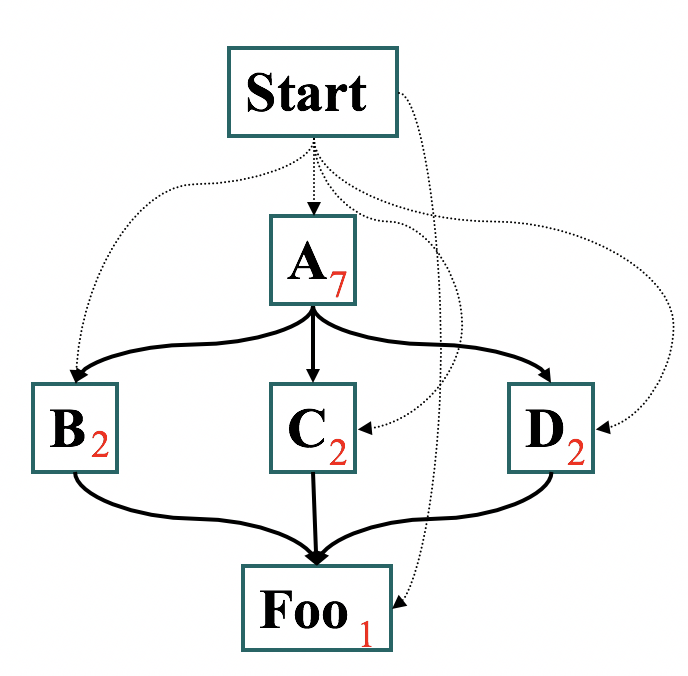
\includegraphics[width=0.4\textwidth]{images/callpaths.png}
\end{center}
\end{changemargin}
\end{frame}



\begin{frame}
\frametitle{Another Call Graph}

\large
Example 2 of relationships between functions.\\
Numbers on edges represent the number of invocations:

\begin{center}
	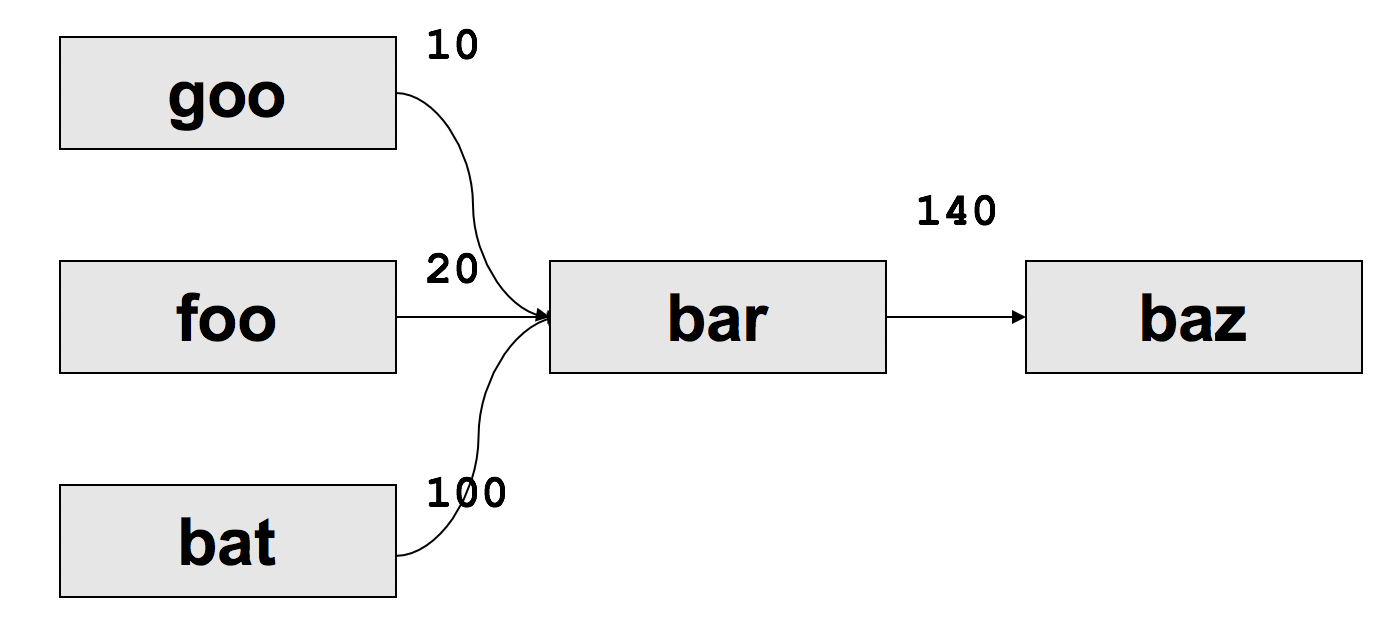
\includegraphics[width=\textwidth]{images/callpaths2.png}
\end{center}

\end{frame}



\begin{frame}
\frametitle{The POGO View of the World}
\large
When considering what to do here, POGO takes the view like this:

\begin{center}
	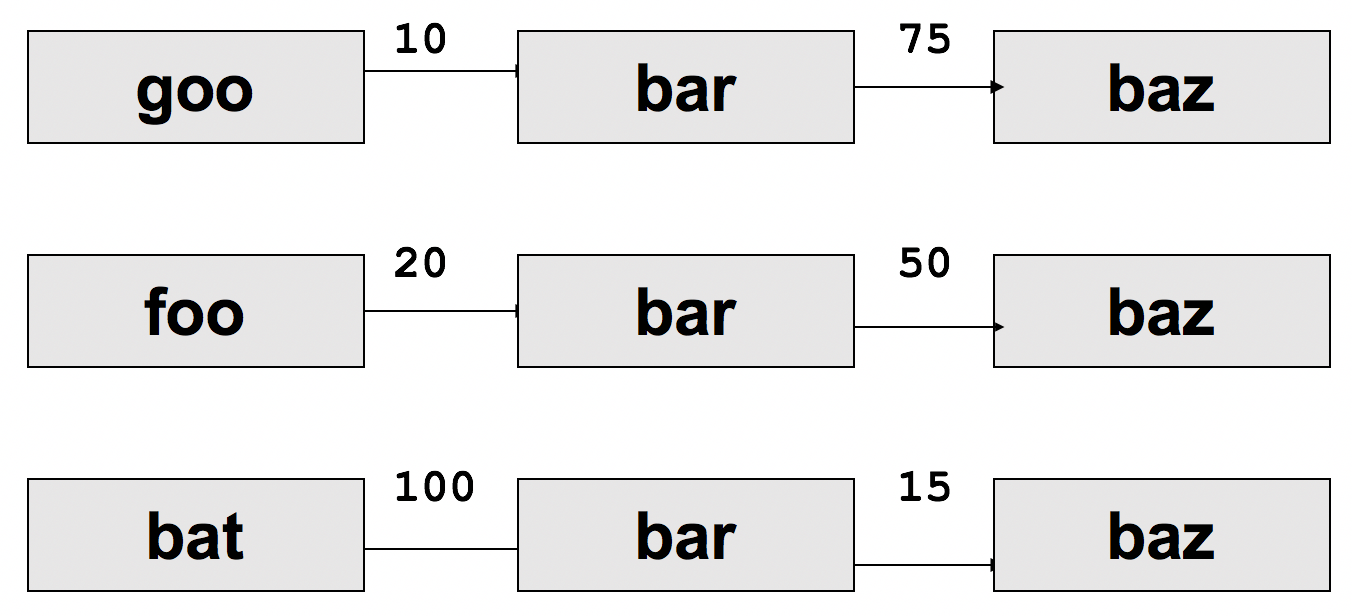
\includegraphics[width=\textwidth]{images/callpaths3.png}
\end{center}

\end{frame}



\begin{frame}
\frametitle{The POGO View of the World}

\begin{center}
	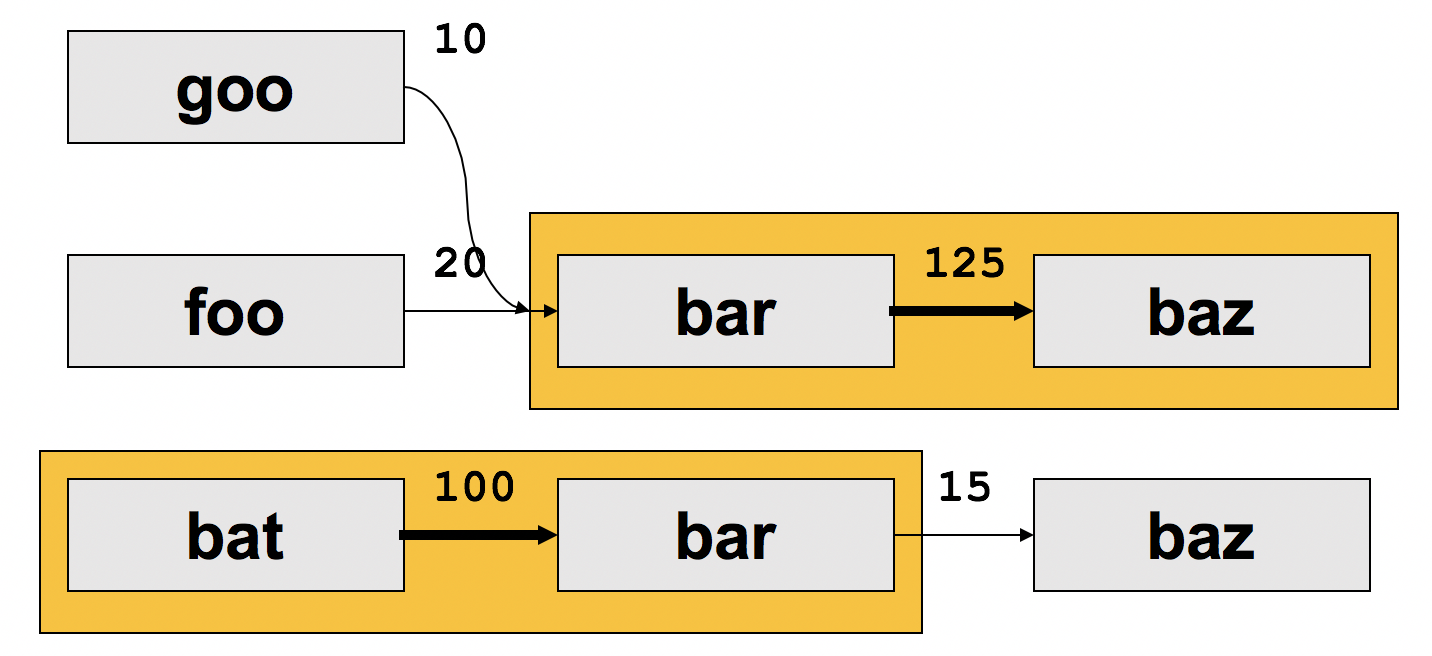
\includegraphics[width=\textwidth]{images/callpaths4.png}
\end{center}

\end{frame}




\begin{frame}
\frametitle{Page Locality}

\large
\begin{changemargin}{1cm}
Call graph profiling data also good for packing blocks.

Put most common cases nearby.\\
Put successors after their predecessors.

Packing related code = fewer page faults (cache misses).

Calling a function in same page as caller =  ``page locality''.
\end{changemargin}

\end{frame}



\begin{frame}
\frametitle{Block Layout}

\begin{center}
	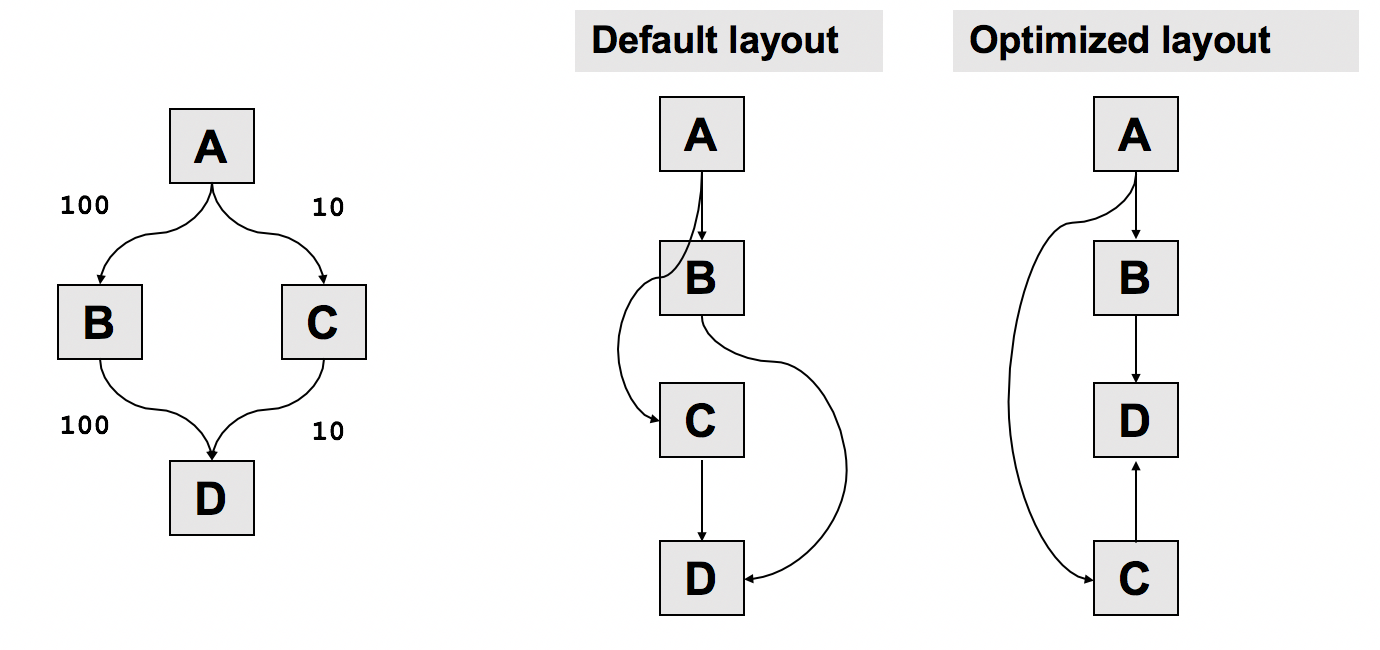
\includegraphics[width=\textwidth]{images/blocklayout.png}
\end{center}

\end{frame}



\begin{frame}
\frametitle{Dead Code?}

\large
\begin{changemargin}{1cm}
According to the author, ``dead'' code goes in its own special block. 

Probably not truly dead code (compile-time unreachable).

Instead: code that never gets invoked in training.
\end{changemargin}

\end{frame}



\begin{frame}
\frametitle{Benchmark Results}
\large \begin{changemargin}{2cm}
OK, how well does POGO work?

The application under test is a standard benchmark suite (Spec2K):
\end{changemargin}

\begin{center}
\begin{tabular}{l|l|l|l|l|l}
	\textbf{Spec2k:} & \textbf{sjeng} & \textbf{gobmk} & \textbf{perl} & \textbf{povray} & \textbf{gcc}\\ \hline
	\textbf{App Size:} &  {Small} & {Medium} & {Medium} & {Medium} & {Large} \\ \hline
	\textbf{Inlined Edge Count} & 50\% & 53\% & 25\% & 79\% & 65\% \\ \hline
	\textbf{Page Locality} & 97\% & 75\% & 85\% & 98\% & 80\% \\ \hline
	\textbf{Speed Gain} & 8.5\% & 6.6\% & 14.9\% & 36.9\% & 7.9\% \\ 
\end{tabular}
\end{center}

\large \begin{changemargin}{2cm}
We can speculate about how well synthetic benchmarks results translate to real-world application performance\ldots
\end{changemargin}

\end{frame}



\end{document}

